% PACKAGES INCLUDED HERE 
% DO NOT NEED TO CHANGE
\documentclass[conference]{IEEEtran}
%\IEEEoverridecommandlockouts
% The preceding line is only needed to identify funding in the first footnote. If that is unneeded, please comment it out.
\usepackage{listings}
\usepackage{csquotes}
\usepackage{float}
\usepackage[caption=false]{subfig}
\usepackage{cite}
\usepackage{amsmath,amssymb,amsfonts}
\usepackage{algorithmic}
\usepackage{graphicx}
\usepackage{textcomp}
\usepackage{hyperref}
\usepackage{url}
\usepackage{amsmath}
\def\BibTeX{{\rm B\kern-.05em{\sc i\kern-.025em b}\kern-.08em
    T\kern-.1667em\lower.7ex\hbox{E}\kern-.125emX}}
\begin{document}

% TITLE GOES HERE

\title{Predicting Pseudo Random Values Using Convolutional Neural Networks\\}


% AUTHOR NAMES GOES HERE


\author{
\IEEEauthorblockN{Najib Ali}
\IEEEauthorblockA{\textit{Department of Computer Science}\\
\textit{Middle Tennessee State University}\\
Murfreesboro, Tennessee \\
email address}\\[0.4cm]  %<------- Extra vertical space
\IEEEauthorblockN{Matthew Hawks}
\IEEEauthorblockA{\textit{Department of Computer Science}\\
\textit{Middle Tennessee State University}\\
Murfreesboro, Tennessee \\
email address}
\and
\IEEEauthorblockN{Jacob Anderson}
\IEEEauthorblockA{\textit{Department of Computer Science}\\
\textit{Middle Tennessee State University}\\
Murfreesboro, Tennessee \\
email address}\\[0.4cm]  %<------- Extra vertical space
\IEEEauthorblockN{Ryan Hines}
\IEEEauthorblockA{\textit{Department of Computer Science}\\
\textit{Middle Tennessee State University}\\
Murfreesboro, Tennessee \\
email address}
\and
\IEEEauthorblockN{Spencer Arnold}
\IEEEauthorblockA{\textit{Department of Computer Science}\\
\textit{Middle Tennessee State University}\\
Murfreesboro, Tennessee \\
email address}\\[0.4cm]  %<------- Extra vertical space
\IEEEauthorblockN{Tae Kweon}
\IEEEauthorblockA{\textit{Department of Computer Science}\\
\textit{Middle Tennessee State University}\\
Murfreesboro, Tennessee \\
email address}
}

\maketitle

% ABSTRACT 

\begin{abstract}
This document is a model and instructions for \LaTeX.
This and the IEEEtran.cls file define the components of your paper [title, text, heads, etc.]. *CRITICAL: Do Not Use Symbols, Special Characters, Footnotes, 
or Math in Paper Title or Abstract.
This document is a model and instructions for \LaTeX.
This and the IEEEtran.cls file define the components of your paper [title, text, heads, etc.]. *CRITICAL: Do Not Use Symbols, Special Characters, Footnotes, 
or Math in Paper Title or Abstract.
This document is a model and instructions for \LaTeX.
This and the IEEEtran.cls file define the components of your paper [title, text, heads, etc.]. *CRITICAL: Do Not Use Symbols, Special Characters, Footnotes, 
or Math in Paper Title or Abstract.
This document is a model and instructions for \LaTeX.
This and the IEEEtran.cls file define the components of your paper [title, text, heads, etc.]. *CRITICAL: Do Not Use Symbols, Special Characters, Footnotes, 
or Math in Paper Title or Abstract.

\end{abstract}


% KEYWORDS

\begin{IEEEkeywords}
component, formatting, style, styling, insert
\end{IEEEkeywords}

% INTRODUCTION SECTION
\section{Introduction}


% BACKGROUND SECTION
\section{Background}


% METHODS SECTION
\section{Methods}
\subsection{Seeding Method}
We went with a seed generation method that allowed a way to introduce some minor level of entropy to avoid letting the neural network aimlessly swim through the entropy of a strong seed instead of gaining stochastic insight on the data from the PRNG.

The seed generation method we chose derives from the concept of using the system time as an element for seed generation. The specific implementation we chose took inspiration from Microsoft's .NET system.datetime.ticks property. \cite{msoftdocs} We chose to single out this method due to its documentation and unique simplicity. System time is widely used as a parameter for modern seed generation methods. 

To put it more trivially: "a pseudo-random number generator is a deterministic algorithm that, given an initial number (called a seed), generates a sequence of numbers that adequately satisfy statistical randomness tests. Since the algorithm is deterministic, the algorithm will always generate the exact same sequence of numbers if it's initialized with the same seed. That's why system time (something that changes all the time) is usually used as the seed for random number generators." \cite{pseudoquote}

According to the Microsoft documentation, "A single tick represents one hundred nanoseconds or one ten-millionth of a second. There are 10,000 ticks in a millisecond, or 10 million ticks in a second. The value of this property represents the number of 100-nanosecond intervals that have elapsed since 12:00:00 midnight, January 1, 0001 in the Gregorian calendar." \cite{msoftdocs}

We used a fairly similar Python port, as seen in Figure ~\ref{fig:Default Seeding Method}

\begin{figure}[H]
\centering
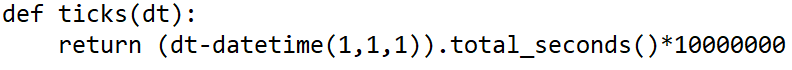
\includegraphics[width=1\linewidth]{./Images/Ticks.png}
\caption{Default Seeding Method}
\label{fig:Default Seeding Method}
\end{figure}

This python port of Microsoft's tick method can be attributed to "mhawke" on StackOverflow. \cite{tickport} The author had some noteworthy comments about this implementation, namely some porting side effects:
\begin{enumerate}
    \item UTC times are assumed.
    \item The resolution of the DateTime object is given by DateTime.resolution, which is DateTime.timedelta(0, 0, 1) or microsecond resolution (1e-06 seconds). CSharp Ticks are purported to be 1e-07 seconds.
\end{enumerate}

For experimental needs, we made additional changes to the implementation:
\begin{enumerate}
    \item Changing start time from January 1, 0001 to January 1, 1970, which effectively reduced the length of the seed for experimental purposes.
    \item Slicing the last 6 digits of the ticks result to acquire more digit variation for frequent invocation.
\end{enumerate}

The final modified method allows enough spread between frequently retrieved ticks, where we are assuming reasonable pseudo-unpredictability. This serves as a simplistic but constantly changing control mechanism for being able to seed PRNGs and test experimental outcomes. While not the most cryptographically strong, we needed a way to have some controlled aspect of seed generation to feed into generators of varying cryptographic complexity (to have some baseline of comparison).

The original idea was to feed each PRNG different seeds from the same seed generator; however, many PRNG algorithms impose strict seed requirements to pass tests of randomness. Out of the five PRNG methods we implemented, Lagged Fibonacci was the only one that had special seed requirements, so we created a separate seed generator based on the same fundamental ticks generation method, but modified to meet the restrictions. Other PRNGs not implemented in this research that impose seed restrictions include Wichmann-Hill (which accepts three different seeds) and Maximally Periodic Reciprocals (which requires a Sophie Prime), among others.

You might ask: won't different seed generators introduce flaws or bias in the experiment? Well, it depends on what you are testing. In our case, we are strictly testing the "complexity" of the generator itself, so supplying a seed that is not blatantly predictable but also not unpredictable was sufficient. Our goal was to allow the characteristics of the generator to be exposed, for we were cracking the "complexity" of the generation algorithm, not the complexity of an arbitrary seed.

\subsection{PRNG Implementations}
For the experiment, we chose five PRNG methods by year of invention. We attempted to choose PRNG methods that displayed popularity in the world of pseudo random number generation while making sure the year of invention was reasonably distributed among the group. Choosing five PRNGs allowed us to focus on implementations, while leaving future research opportunities open for working with other PRNGs that we did not cover.

Chosen PRNGs:
\begin{itemize}
  \item Middle-square method (1946)
  \item Linear congruential generator (1958)
  \item Lagged Fibonacci (1965)
  \item Park-Miller (1988)
  \item Mersenne Twister (1998)
\end{itemize}

The call definition of any given PRNG function is as follows:
\begin{lstlisting}
PRNGfunc(seed, n) 
\end{lstlisting}
This is so we can experimentally automate the calling of each PRNG without getting too complex.
The given PRNG function should return a list of n generated numbers using the generation method.
All other parameters outside of the seed and n are default values.

For example, if the call was PRNG(seed, 10),
it might return something like
[3,5,10,1,31,17,2,4,6,7]

We control parsing the n-length list and handling seeds externally. 
This plays logically with separation of concerns for our usecase.

While python generators can be useful iterating over previously generated iterables,
we did not want to clutter our experimental execution code, so we stuck to a classical
internal handling of all iterations.

Below are short descriptions of each PRNG and any implementation notes made during the developement process.
Middle Square:
Description:
...
Notes:
A note on weakness: For a generator of n-digit numbers, the period can be no longer than 8n. If the middle n digits are all zeroes, 
the generator then outputs zeroes forever. If the first half of a number in the sequence is zeroes, the subsequent
numbers will be decreasing to zero. While these runs of zero are easy to detect, they occur too frequently for this
method to be of practical use. The middle-squared method can also get stuck on a number other than zero.

An already seen list is NOT included in the original middle square method and will not be used.

Linear Congruential:
Description:
...
Notes:
The generator is not sensitive to the choice of c, 
as long as it is relatively prime to the modulus 
(e.g. if m is a power of 2, then c must be odd), 
so the value c=1 is commonly chosen.

If c = 0, the generator is often called a multiplicative
congruential generator (MCG), or Lehmer RNG. If c ≠ 0, the
method is called a mixed congruential generator.

Parameters were chosen based on $2^32$ in table 2 of 
\url{https://citeseerx.ist.psu.edu/viewdoc/download;jsessionid=BBA0C7ED3ADAB606642BB8D939774B4F?doi=10.1.1.34.1024&rep=rep1&type=pdf}

Lagged Fibonacci:
Description:
...
Notes:
This is two tap, not three tap...
It's a "lagged" generator, because "j" and "k" lag behind the generated pseudorandom value. 
Also, this is called a "two-tap" generator, in that you are using 2 values in the sequence 
to generate the pseudorandom number. However, a two-tap generator has some problems with 
randomness tests, such as the Birthday Spacings. Apparently, creating a "three-tap" generator
addresses this problem.

Park Miller:
Description:
...
Notes:
The Lehmer generator is an lcg. Park Miller is a specific lcg.
    
The Lehmer random number generator (named after D. H. Lehmer), 
sometimes also referred to as the Park–Miller random number generator
(after Stephen K. Park and Keith W. Miller), is a type of linear congruential generator (LCG).

Park miller generator, because they essentially the same.
Park-miller request the use of certain modulos.
Lehmer is an lcg where c = 0...
If c = 0, the generator is often called a multiplicative congruential generator (MCG),
or Lehmer RNG. If c ≠ 0, the method is called a mixed congruential generator.

While the Lehmer RNG can be viewed as a particular case of the linear congruential generator
with c=0, it is a special case that implies certain restrictions and properties.
In particular, for the Lehmer RNG, the initial seed must be coprime to the modulus m that is
not required for LCGs in general. 

The choice of the modulus m and the multiplier a is also more restrictive for the Lehmer RNG.
In contrast to LCG, the maximum period of the Lehmer RNG equals m−1 and it is such when m is 
prime and a is a primitive root modulo m. 

Mersenne Twister:
Description:
...
Notes:
Closely related with LFSRs. In its MT19937 implementation is probably the most commonly used modern PRNG. 
Default generator in the Python language starting from version 2.3. 

We used numpy's version of the Mersenne Twister.

\subsection{Experimental Setup}


The following is a vastly informal mathematical representation of our experimental model, using a loose coupling of TLA+ notation and some set-builder theory. Further explanations and graphics will follow to aide in interpretation of the design of the experimental setup.

\begin{displayquote}
Let $n$ be any arbitrary natural number such that $\{n \in \mathbb{N}\}$.
Let $E$ represent the experiment definition.
Let $seed$ be a function such that when called will return a seed.
Given $k$ and $S_n$, let $prng$ be a function such that when called will return a set of pseudo random numbers,
dervied from an initial seed $S_n$ and a given algorithm, where the length of the set is $k$.
\end{displayquote}

\begin{figure}[H]
\centering
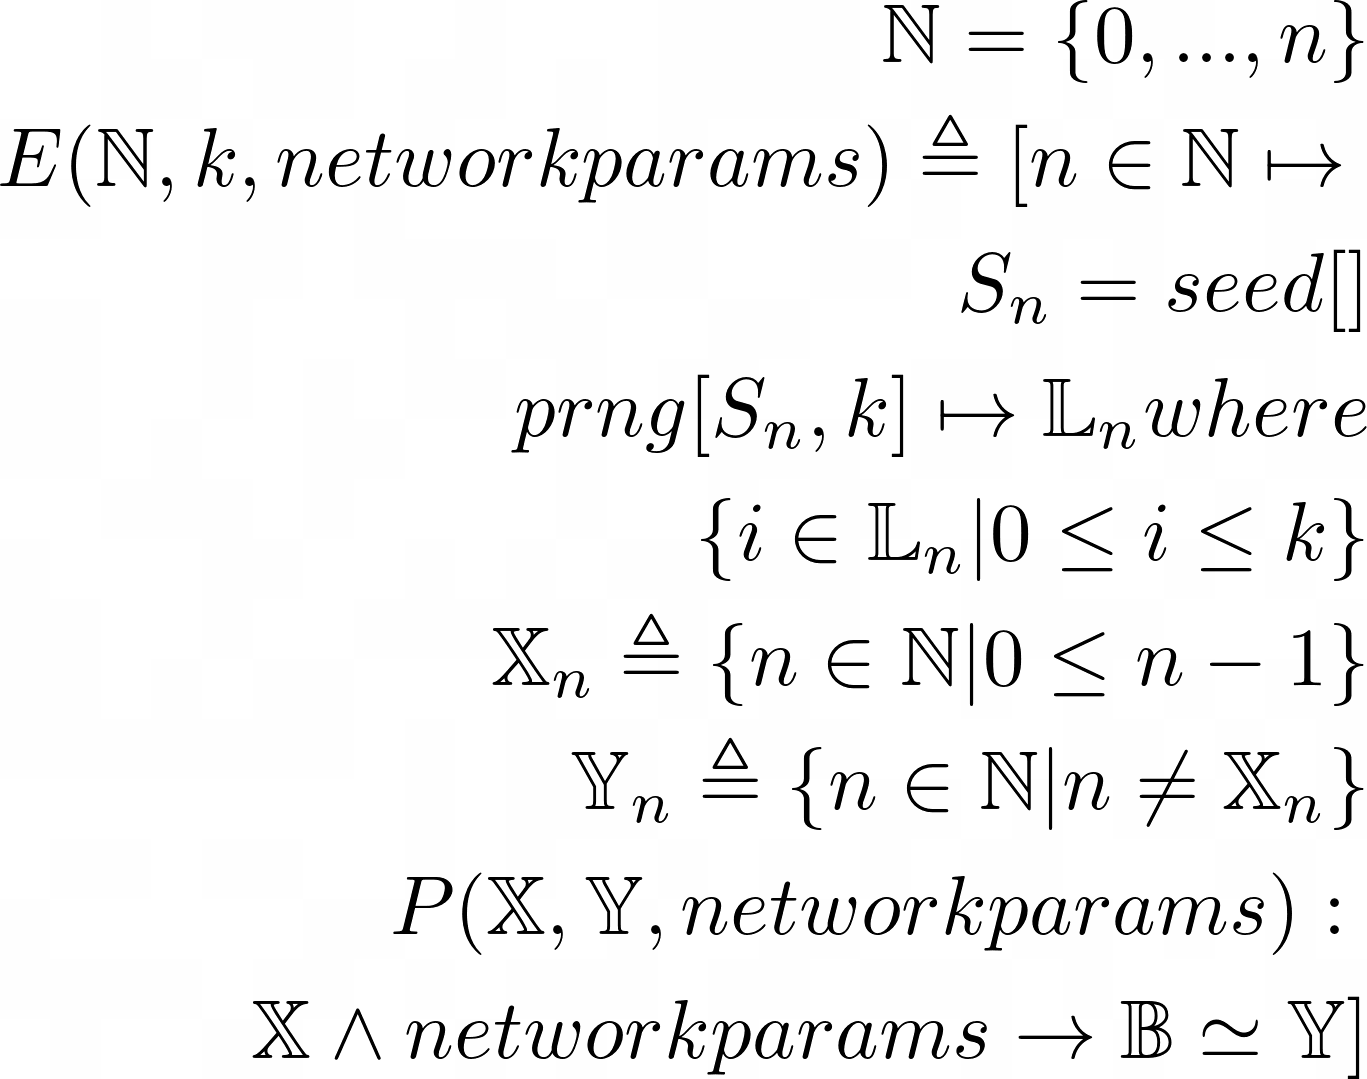
\includegraphics[width=.5\linewidth]{./Images/ModelNotated.png}
\caption{Notated Experiment Model}
\label{fig:Notated Experiment Model}
\end{figure}


Given an enumerated set, $\mathbb{N}$,
where $prng$ is the chosen PRNG, $S_n$ is nth seed in the iteration, and $k$ is the length of the desired output vector ($\mathbb{L}_n$) of $prng$,
$\mathbb{X}_n$ represents an enumerated set containing $n$ sets of $k-1$ values generated from a PRNG ($prng$) and each $\mathbb{X}_n$ set is dervied from a different seed. $\mathbb{Y}_n$ represents a set containing $n$ sets of $k$th values with a direct mapping to each $\mathbb{X}_n$ such that $\mathbb{X}_n \mapsto \mathbb{Y}_n$. $P$ a predictor function that represents a convolutional neural network, which takes in $\mathbb{X}_n$ and $\mathbb{Y}_n$, yields a new set $\mathbb{B}_n$ implied from $\mathbb{X}_n$, where the model trains $\mathbb{B}_n$ to be similar or equal to $\mathbb{Y}_n$ based on back-propagation due to previous predictions, thus using supervised learning to build a regression model.

For a simplified graphical representation of the latter description, please reference the predictive model in Figure ~\ref{fig:Predictive Model}, the simplified experimental model in Figure ~\ref{fig:Simplified Experimental Model} , and the granular view of the experimental model in Figure ~\ref{fig:Granular Experimental Model}.


\begin{figure}[H]
\centering
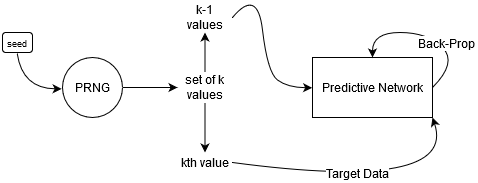
\includegraphics[width=1\linewidth]{./Images/SimpleModel.png}
\caption{Simplified Experimental Model}
\label{fig:Simplified Experimental Model}
\end{figure}

Referencing Figure ~\ref{fig:Simplified Experimental Model}, which is a visualization of what a 1-dimensional architecture of our experiment might entail, the predictive neural net as visualized in Figure ~\ref{fig:Predictive Model} is fed outputs of a specific PRNG, which will attempt to predict an kth value, based on previous k-1 values in a particular set of input data, where each set is generated based off of a single unique seed. After being trained on, ideally thousands of sets, the predictive network will form a better stochastic "understanding" of how the PRNG works underneath, thus being able to more accurately predict numbers generated from that PRNG in the future (i.e.,a supervised regression model). The backpropagation will flow through the predictive network to acheive the adversarial nature of a traditional GAN setup, but in reality, we won't be using a generative network, but rather a PRNG algorithm, so the generative part of our setup won't be defensive.


\begin{figure}[H]
\centering
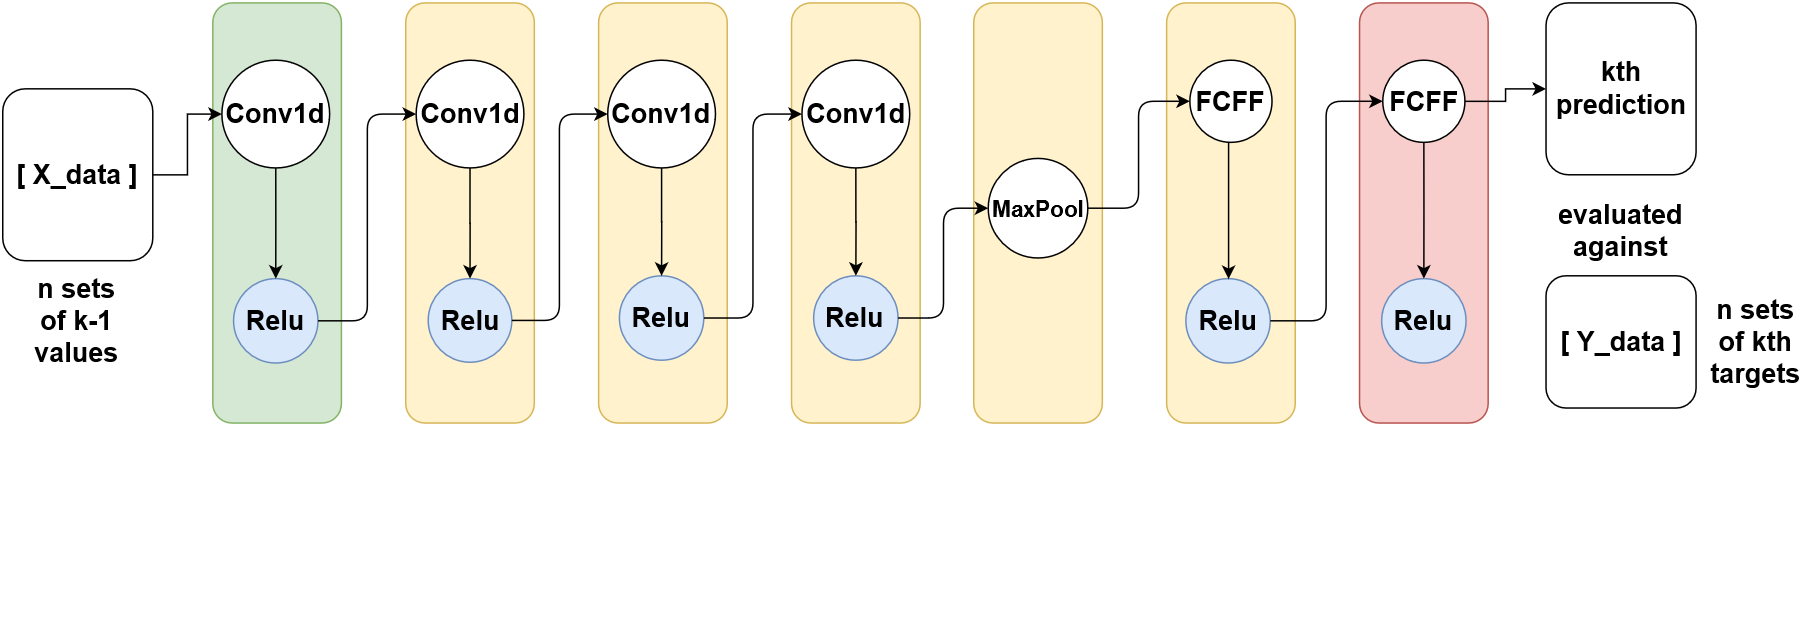
\includegraphics[width=1\linewidth]{./Images/PredictiveModel.png}
\caption{Predictive Model}
\label{fig:Predictive Model}
\end{figure}

Referencing Figure ~\ref{fig:Predictive Model}, which is a visualization of the layer stack we used for the predictive network in each trial of the experiment, it "consists of four stacked convolutional layers, each with 4 filters, kernel size 2, and stride 1, followed by a max pooling layer and two FCFFlayers with 4 and 1 units, respectively. The stack of convolutional layers allow the network to discover complex patterns in the input." [https://arxiv.org/pdf/1810.00378.pdf] Explain here how/why we used that research's dicriminator model in our experiment exactly, except we implemented Relus instead of leaky-relus. Talk about the input xdata and ydata shape and reference the granular model Figure ~\ref{fig:Granular Experimental Model} for detail on how these data are aggregated.



\begin{figure}[H]
\centering
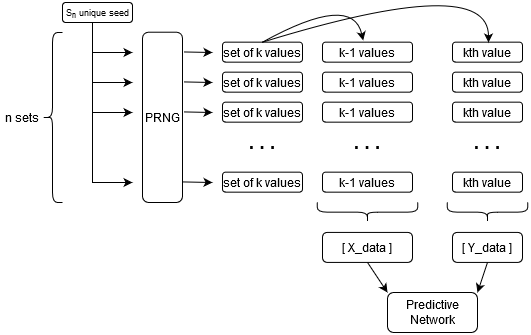
\includegraphics[width=1\linewidth]{./Images/GranularModel.png}
\caption{Granular Experimental Model}
\label{fig:Granular Experimental Model}
\end{figure}

Talk generally about the data aggregation process, just walk through it.

\subsection{Experimental Execution}
Highlight configuration parameters used to execute the experiment.
Make a note the reasoning behind our small num of epochs and general reasoning behind all parameters. 


% RESULTS SECTION
\section{Results}

\begin{figure}[H]
\centering
\subfloat[Subfigure 1 list of figures text][Testing Regression Plot]{
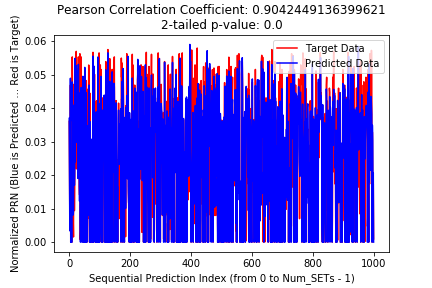
\includegraphics[width=0.4\linewidth]{./Images/Middle_Square_Reg.png}
\label{fig:MS_A}}
\qquad
\subfloat[Subfigure 2 list of figures text][Training Loss Plot]{
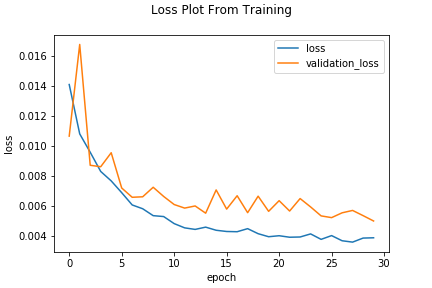
\includegraphics[width=0.4\linewidth]{./Images/Middle_Square_Loss.png}
\label{fig:MS_B}}
\caption{Middle Square Results}
\label{fig:MS}
\end{figure}

\begin{figure}[H]
\centering
\subfloat[Subfigure 1 list of figures text][Testing Regression Plot]{
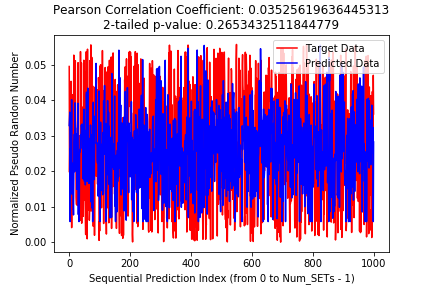
\includegraphics[width=0.4\linewidth]{./Images/Linear_Cong_Reg.png}
\label{fig:LCG_A}}
\qquad
\subfloat[Subfigure 2 list of figures text][Training Loss Plot]{
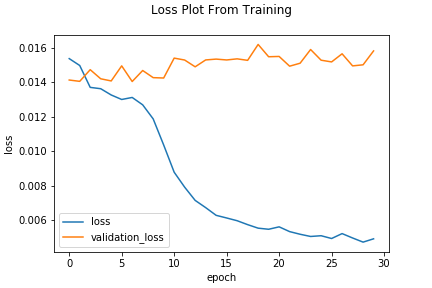
\includegraphics[width=0.4\linewidth]{./Images/Linear_Cong_Loss.png}
\label{fig:LCG_B}}
\caption{Linear Congruential Results}
\label{fig:LCG}
\end{figure}

\begin{figure}[H]
\centering
\subfloat[Subfigure 1 list of figures text][Testing Regression Plot]{
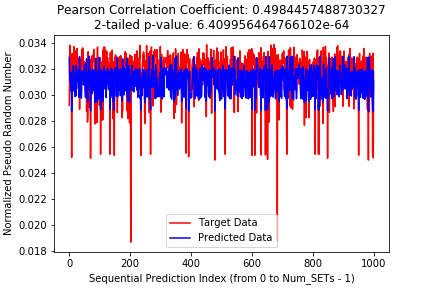
\includegraphics[width=0.4\linewidth]{./Images/Lagged_Fib_Reg.png}
\label{fig:LF_A}}
\qquad
\subfloat[Subfigure 2 list of figures text][Training Loss Plot]{
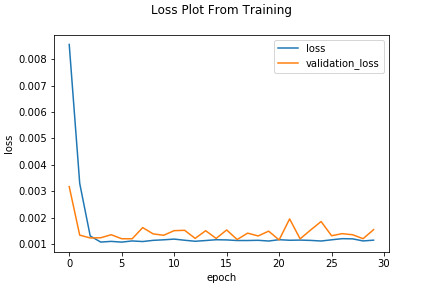
\includegraphics[width=0.4\linewidth]{./Images/Lagged_Fib_Loss.png}
\label{fig:LF_B}}
\caption{Lagged Fibonacci Results}
\label{fig:LF}
\end{figure}

\begin{figure}[H]
\centering
\subfloat[Subfigure 1 list of figures text][Testing Regression Plot]{
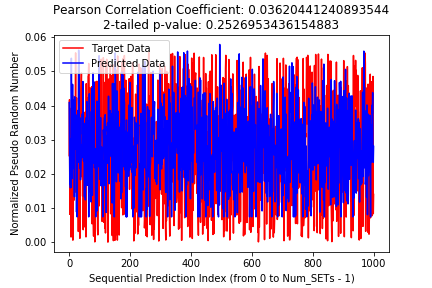
\includegraphics[width=0.4\linewidth]{./Images/Park_Miller_Reg.png}
\label{fig:PM_A}}
\qquad
\subfloat[Subfigure 2 list of figures text][Training Loss Plot]{
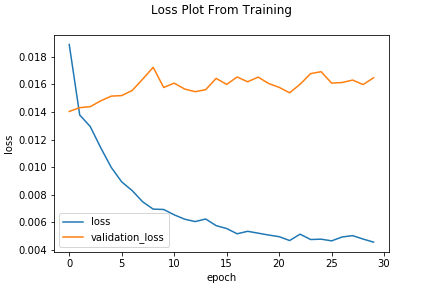
\includegraphics[width=0.4\linewidth]{./Images/Park_Miller_Loss.png}
\label{fig:PM_B}}
\caption{Park Miller Results}
\label{fig:PM}
\end{figure}

\begin{figure}[H]
\centering
\subfloat[Subfigure 1 list of figures text][Testing Regression Plot]{
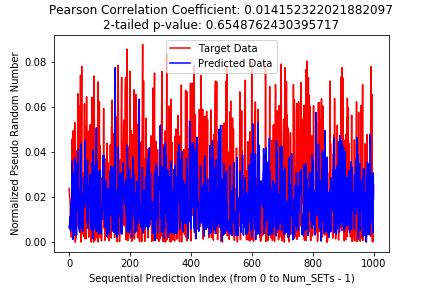
\includegraphics[width=0.4\linewidth]{./Images/Twister_Reg.png}
\label{fig:MT_A}}
\qquad
\subfloat[Subfigure 2 list of figures text][Training Loss Plot]{
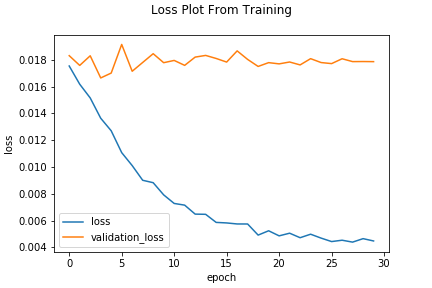
\includegraphics[width=0.4\linewidth]{./Images/Twister_Loss.png}
\label{fig:MT_B}}
\caption{Mersenne Twister Results}
\label{fig:MT}
\end{figure}

% DISCUSSION SECTION
\section{Discussion}
Start typing here her is Start typing here her isStart typing here her isStart typing here her isStart typing here her isStart typing here her isStart typing here her isStart typing here her isStart typing here her isStart typing here her isStart typing here her isStart typing here her isStart typing here her isStart typing here her isStart typing here her isStart typing here her isStart typing here her isStart typing here her isStart typing here her isStart typing here her isStart typing here her isStart typing here her isStart typing here her isStart typing here her isStart typing here her isStart typing here her isStart typing here her isStart typing here her isStart typing here her isStart typing here her is

.. code:: ipython3

    % REFERENCES
    % THIS IS CREATED AUTOMATICALLY
    \bibliographystyle{IEEEtran}
    \bibliography{References} % change if another name is used for References file

\end{document}
